\subsection{Statistics of Binary Classifiers}

Evaluating the performance of the feature matching algorithms on the converted depth images is done by analyzing the matching process as a binary classifier.
The clasification task is to determine if a keypoint $\mathbf{K_1}$ of image $I_1$ corresponds with keypoint $\mathbf{K_2}$ in image $I_2$ with a binary outcome.
A pair of keypoints corresponds, if both pixel coordinates projected into space intersect at the same point, allowing for a little bit of uncertainty, e.g. $2px$ backprojection difference.

As with most statistics it is necessary to consider the distribution of a quantity and analyze it from multiple view points.
Therefore, the final evaluation will consider other criteria, like keypoint distribution and number of keypoints per frame.

Pairs of keypoints are defined as \emph{positive} ($P$) if they correspond and \emph{negative} ($N$) otherwise.
The predicted outcome of the matching system is either \emph{yes} ($y$) or \emph{no} ($n$).

The result of this prediction is in one of four categories.
A correspondence can be correctly, a \emph{true positive} ($TP$), or mistakenly recognized, a \emph{false positive} ($FP$).
Similarly, the lack of correspondence can be either correctly or incorrectly, so called \emph{true negatives} ($TN$) and \emph{false negatives} ($FN$), detected.
The \emph{confusion matrix}, a specialized case of a \emph{contingency table}\cite{agresti_2007}, keeps track of classification outcomes and is the basis for many performance criteria and derived metrics.
Table~\ref{tab:def_confusion_matrix} demonstrates the arrangement of elements in a confusion matrix.
The provided values can be either an absolute count of elements or a relative share of total elements and must be exhaustive.

\begin{table}
\bgroup%
\def\arraystretch{1.5}%  1 is the default, change whatever you need
\setlength\tabcolsep{0.5em}
\begin{tabular}{r|c|c|l}
    \multicolumn{1}{r}{} &
    \multicolumn{1}{c}{$P$} &
    \multicolumn{1}{c}{$N$} &
    \multicolumn{1}{l}{} \\
  \cline{2-3}
  $y$ & $TP$  & $FP$ & Total \emph{yes} \\
  \cline{2-3}
  $n$ & $FN$  & $TN$ & Total \emph{no} \\
  \cline{2-3}
    \multicolumn{1}{r}{} &
    \multicolumn{1}{c}{Total \emph{Positives} ($\#P$)} &
    \multicolumn{1}{c}{Total \emph{Negatives} ($\#N$)}
\end{tabular}
\egroup%
\caption[Definition of the Confusion Matrix]{A confusion matrix summarizes the decision quality of a binary classifier. The elements to be classified can be in either category; \emph{positive} ($P$) or \emph{negative} ($N$). Correct classifications of elements are either \emph{true positives} ($TP$) or \emph{true negatives} ($TN$). Missclassification results in \emph{false positives} ($FP$) or \emph{false negatives} ($FN$).}\label{tab:def_confusion_matrix}
\end{table}

All \emph{positive} elements are \emph{relevant elements} in the sense, that the keypoint pair points to the same world coordinate.
Predicted correspondences ($y$) are called \emph{selected elements}.
Different common ratios are derived from the confusion matrix.

\begin{description}
    \item[True Positive Rate] The true positive rate defines the ratio of correctly identified positive elements to total positive elements and is also called \textbf{hit rate}, \textbf{recall} or \textbf{sensitivity}.
        \begin{equation}
            TPR = \frac{TP}{\#P}
            \label{eq:true_positive_rate}
        \end{equation}
    \item[False Positive Rate] This ratio shows how many negative elements are mistakenly classified as positive elements. It is sometimes named \textbf{false alarm rate} or \textbf{fallout}.
        \begin{equation}
            FPR = \frac{FP}{\#N}
            \label{eq:false_positive_rate}
        \end{equation}
    \item[True Negative Rate] Also called \textbf{specificity}, the true negative rate is the ratio of correctly rejected elements.
        \begin{equation}
        \begin{aligned}
            TNR &= \frac{TN}{\#N} \\
                &= 1 - FPR
        \end{aligned}
        \label{eq:true_negative_rate}
        \end{equation}
    \item[Accuracy] The accuracy is the percentage of correctly classified elements. This measure is called \textbf{Rand index} in data clustering.
        \begin{equation}
            A = \frac{TP + TN}{\#P + \#N} = \frac{TP + TN}{TP + FP + TN + FN}
            \label{eq:accuracy}
        \end{equation}
    \item[Precision] The precision is the ratio of positive elements in all selected elements.
        \begin{equation}
            precision = \frac{TP}{TP + FP}
        \end{equation}
\end{description}
Each of these ratios can be of any value between $[0, 1]$ and might be written as a percentage.
Both precision and recall are commonly used to compare and evalute feature matching algorithms and keypoint descriptors.
The proposed metric share the pitfall, that a low number of total elements or highly skeweed data can result in very strong results for each metric, but correspond to a weak real world performance.

\subsubsection{Receiver Operating Statistics Analysis}

Choosing a suitable configuration or algorithm combination requires trade-offs between different aspects of the final system.
Receiver Operating Statistics (ROC) analysis\cite{fawcett_2006} provides a tool to visualize the trade-offs between different systems.
The central component of this analysis are the \emph{ROC graphs}.
They plot the false positive rate and true positive rate, the \emph{ROC space}, of multiple classifiers in one graph, with figure~\ref{fig:roc_graph} containing all qualitatively different cases.
\begin{figure}[H]
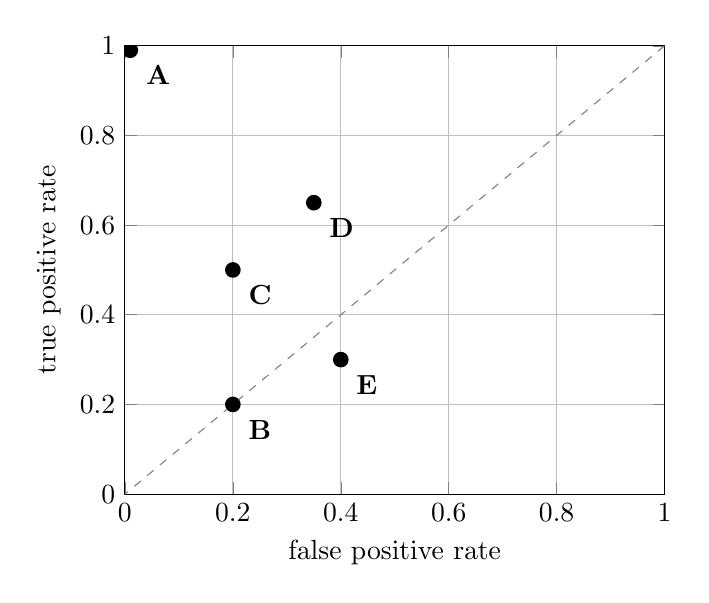
\begin{tikzpicture}
\begin{axis}[xmin=0,xmax=1,ymin=0,ymax=1,samples=50,xlabel={false positive rate}, ylabel={true positive rate},grid=major]
  \addplot[gray, dashed] (x,x);
  \node[label={315:{$\mathbf{A}$}},circle,fill,inner sep=2pt] at (axis cs:0.01,0.99) {};
  \node[label={315:{$\mathbf{B}$}},circle,fill,inner sep=2pt] at (axis cs:0.2,0.2) {};
  \node[label={315:{$\mathbf{C}$}},circle,fill,inner sep=2pt] at (axis cs:0.2,0.5) {};
  \node[label={315:{$\mathbf{D}$}},circle,fill,inner sep=2pt] at (axis cs:0.35,0.65) {};
  \node[label={315:{$\mathbf{E}$}},circle,fill,inner sep=2pt] at (axis cs:0.4,0.3) {};
\end{axis}
\end{tikzpicture}
\caption[The elements of a ROC graph]{A ROC graph plots the true positive rate versus the false positive rate of a binary classifier. Each point is one classification system. The diagonal $f(x) = x$ is equivalent to a 50\% chance of correct classification and a system on this line has no predictive power, as in this case $\mathbf{B}$. Points above this line ($\mathbf{C}$, $\mathbf{D}$) indicate better-than-random performance and the bigger the distance to this diagonal the higher the informedness, also called Youden-Index, of this system. The optimal classifier ($\mathbf{A}$) is in the topleft corner and has no false decisions. Points below the diagonal ($\mathbf{E}$) might still have predictive power but indicate a wrong labeling of the outcomes.}\label{fig:roc_graph}
\end{figure}

Points above the diagonal have predictive power proportional to the distance to the diagonal.
This distance is also called the \textbf{Youden-Index} $\mathbf{J}$\cite{youden_cancer1950} and is a measure of informedness of the classifier.
\begin{equation}
\begin{aligned}
    J &= sensitivity + specificity - 1
      &= \frac{TP}{TP + FN} + \frac{TN}{TN + FP} - 1
\end{aligned}
\label{eq:youden}
\end{equation}
Unless there are no samples tested, the Youden-Index is $\mathbf{J} \in [0, 1]$.
The higher $\mathbf{J}$ the better the two groups are separated by the classifier.
ROC analysis gives a valueable instrument to compare the relative performance of classifiers.
A final judgement requires to take additional measures like absolute number of classified elements into account.
Fawcett's\cite{fawcett_2006} work provides a more detailed introduction to ROC analysis in machine learning.
